\chapter{Docker Volume}
\section{Pembuka}
Dikutip dari situs Docker Docs, Docker volume merupakan salah satu cara untuk memanage data di docker selain menggunakan Bind Mount. Dengan volume pengguna dapat menyimpan file pada host machine yang dapat diterapkan ke container, sehingga file tetap tersedia meskipun container dihapus. 
Volume disimpan di file host system yang dikelola oleh docker (/var/lib/docker/volumes). Saat membuat docker volume, folder ini akan menyimpan data docker volume. Saat mount volume ke dalam container,
direktori ini yang di mount ke dalam container. Docker menyediakan 2 opsi sintaks untuk membuat volume yaitu -v/--volume dan --mount. Pada kesempatan kali ini akan menggunakan opsi -v/--volume


\section{Kapan menggunakan volume ?}
\begin{itemize}
    \item Berbagi data diantara beberapa container yang sedang berjalan
    \item Menyimpan data container di remote host atau provider
    \item Perlu mencadangkan (backup), memulihkan (restore), atau memigrasikan (migrate) data dari satu docker host ke docker host lain
    \item Aplikasi membutuhkan I/O berkinerja di Docker Desktop
    \item Aplikasi memerlukan perilaku native filesystem di Docker Desktop
\end{itemize}

\begin{figure}
    \begin{center}
        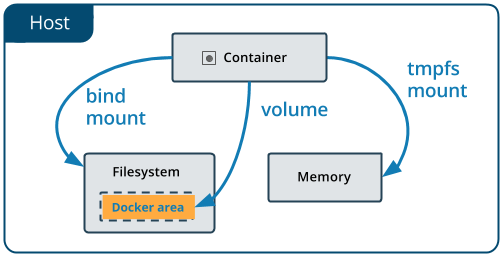
\includegraphics[width=\linewidth]{image/volume.png}
        \caption{Docker Volume}
        \label{fig:my_figure}
    \end{center}
    
    \section{Membuat docker Volume}
    1. Membuat docker volume saat container dibuat
    
    Membuat docker volume saat container dibuat : \textcolor{Gray}{docker run <OPTION> -v <NAMA VOLUME:MOUNT DIREKTORI CONTAINER> --name <NAMA CONTAINER> <NAMA IMAGE>}
    
    COMMAND: \textcolor{Blue}{docker run -dp 80:80 -v volume1:/usr/share/nginx/html --name web nginx:stable-alpine}
    
    Jika sudah cek Volume apakah sudah terbuat
    
    COMMAND: \textcolor{Blue}{docker volume ls}
    
    Lalu cek container apakah berjalan
    
    COMMAND: \textcolor{Blue}{docker ps -a}
    \begin{center}
        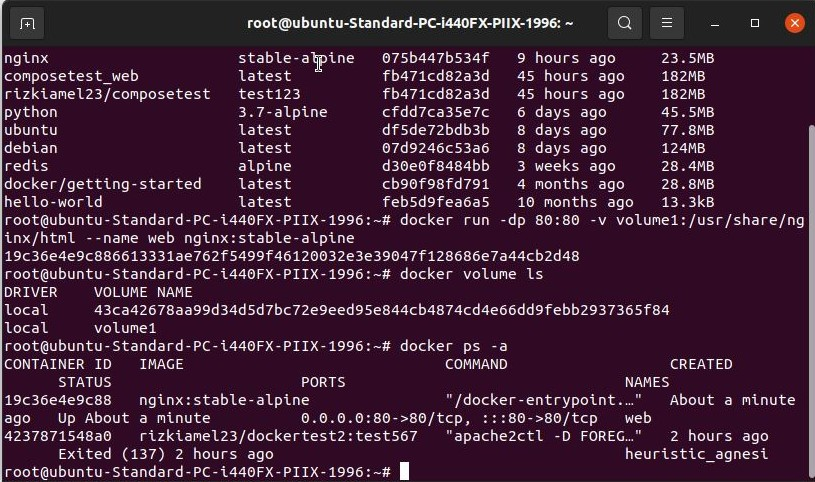
\includegraphics[width=\linewidth]{image/38.jpg}
        \caption{Buat docker volume saat container dibuat}
        \label{fig:my_figure}
    \end{center}

    
\end{figure}
\begin{figure}
    2. Buka browser akes http://0.0.0.0:80, akan muncul tampilan berikut 
    \begin{center}
        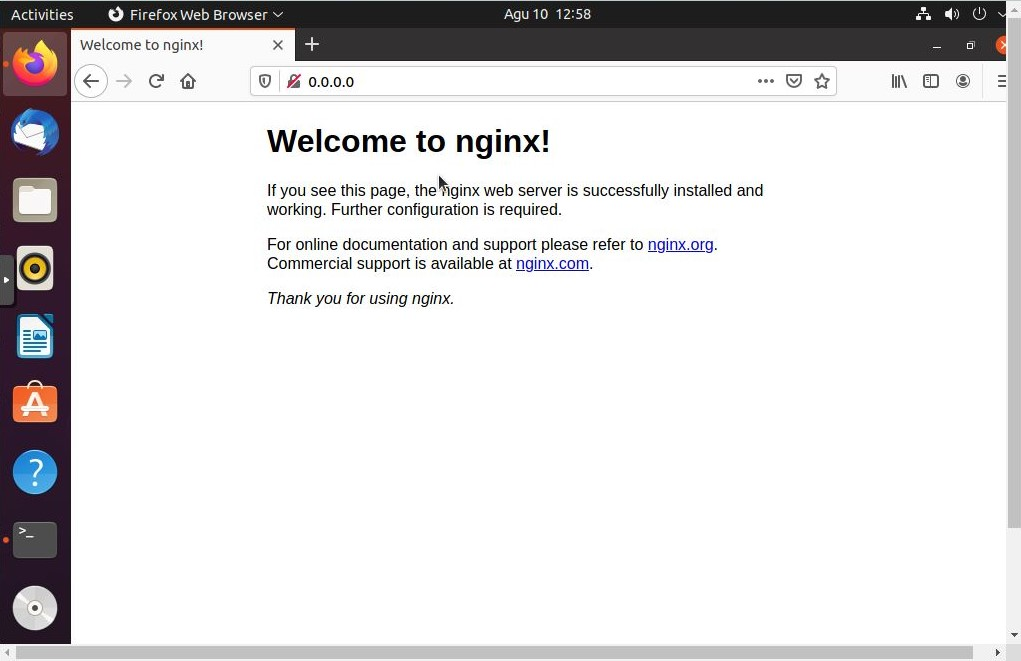
\includegraphics[width=\linewidth]{image/39.jpg}
        \caption{Tampilan mengakses kontainer dalam volume}
        \label{fig:my_figure}
    \end{center}

    3. Periksa detail docker volume
    
    Periksa detail docker volume : \textcolor{Gray}{docker volume inspect <NAMA VOLUME>}
    
    COMMAND: \textcolor{Blue}{docker volume inspect volume1}
    \begin{center}
        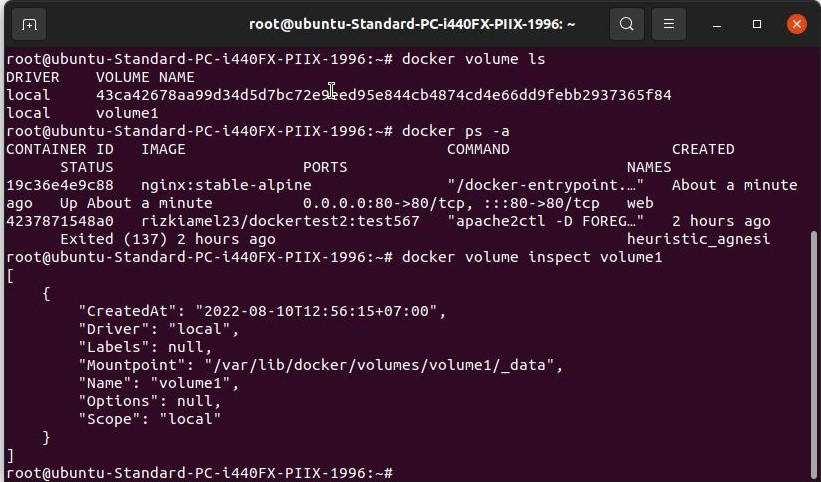
\includegraphics[width=\linewidth]{image/40.jpg}
        \caption{Tampilan inspect docker volume}
        \label{fig:my_figure}
    \end{center}
\end{figure}


